% Provenance (never printed): see sources/outline_sources.md (Year 3: the main
% field and its secular variation, rock magnetism, palaeomagnetic poles, apparent
% polar wander, magnetostratigraphy, the geodynamo). Brief: sources/book5/BRIEFS.md,
% ch. 4. Curves and maps from figdata/bachelor-3/igrf_field.py (IGRF-14),
% palaeomag_stats.py (the invented Kesta terrane, its Fisher statistics, the
% Zijderveld specimen and the reference APW path), magnetostratigraphy.py.
% Exercise and problem values in the Book 5 scratch calculator calc/ch04.py.
\chapter{Geomagnetisme en paleomagnetisme}\label{ch:b3:palaeomagnetism}

Een basaltstroom die zestig miljoen jaar geleden uitbarstte, koelde af
met zijn piepkleine magnetietkorrels vastgelegd evenwijdig aan het veld van die tijd. Vandaag geboord, ter plaatse
georiënteerd, in kleine cilinders gezaagd en
stap voor stap verhit in een kamer die is afgeschermd van het huidige veld, vertelt hij nog steeds
hoe ver hij toen van de pool lag en welke kant hij op wees. Duizenden zulke
metingen, van elk continent en uit elke tijd, hebben laten zien hoe de continenten
bewogen voordat de oceaanbodems ontstonden die hun beweging registreren, en in
welke volgorde het veld is omgekeerd door de lagen van een sedimentaire
sectie heen. Dit hoofdstuk beschrijft het veld zoals het er vandaag uitziet, hoe gesteenten
het vastleggen, hoe een richting wordt bepaald en gemiddeld, en wat een paleomagnetische pool
zegt over de beweging van een plaat.

\begin{recall}
De Aarde als magneet en de magnetische declinatie staan in de
schoolboeken van de natuurkundeboeken; magnetische domeinen, hysterese, remanentie en de Curietemperatuur
in hun Boek~3; het veld van een magnetische dipool in hun
Boek~1. Magnetische omkeringen en de normale en omgekeerde polariteiten
kwamen aan bod in leerjaar~11. De grootcirkel en de bolvormige driehoek werden
gedefinieerd in Boek~1, in het hoofdstuk over bolastronomie; het polariteitschron,
de geomagnetische polariteitsschaal, de marien magnetische anomalie en eindige
rotaties om een Eulerpool in het hoofdstuk over plaatkinematica op een bol;
het hotspotspoor in het hoofdstuk over hotspots. Sferische harmonischen en de
Schmidt-genormaliseerde Legendre-functies $P_n^m$ werden voor de zwaartekracht gebruikt in het
hoofdstuk over zwaartekracht en de vorm van de Aarde (zie \cref{ch:b3:gravity-geodesy}).
\end{recall}

\section{Het hoofdveld}

\begin{definition}[Geomagnetisch hoofdveld; geocentrische axiale dipool]\label{def:b3:palaeomagnetism:main-field}
Het \emph{geomagnetisch hoofdveld}\index{geomagnetisch hoofdveld} is het deel van
het magnetisch veld van de Aarde dat binnen de Aarde wordt opgewekt, in de vloeibare ijzeren
buitenkern; het verandert over jaren tot miljoenen jaren, anders dan de velden van de
ionosfeer en de magnetosfeer, die over seconden tot dagen veranderen. De
\emph{geocentrische axiale dipool}\index{geocentrische axiale dipool} is het veld van een
magnetische dipool die in het middelpunt van de Aarde is geplaatst en met zijn rotatieas is
uitgelijnd, wijzend naar het zuiden, zodat de veldlijnen het zuidelijk halfrond verlaten en
het noordelijk halfrond binnengaan.
\end{definition}

Op elk punt van het oppervlak is het veld $\mathbf F$ een vector. Het wordt
beschreven in een lokaal assenstelsel (figuur hieronder): $X$ naar geografisch noord, $Y$ naar het
oosten, $Z$ naar beneden. Zijn horizontale component is $H = \sqrt{X^2 + Y^2}$, zijn
totale intensiteit $F = |\mathbf F|$, zijn magnetische declinatie $D$ de hoek van
geografisch noord naar $\mathbf H$, rechtsom geteld, en zijn inclinatie $I$ de
hoek van de horizontaal naar $\mathbf F$.

\begin{definition}[Magnetische inclinatie]\label{def:b3:palaeomagnetism:inclination}
De \emph{magnetische inclinatie}\index{magnetische inclinatie} $I$ van het veld op
een punt is de hoek tussen de veldvector en het horizontale vlak,
positief wanneer het veld naar beneden wijst: $\tan I = Z/H$, met $-\ang{90} \le I
\le \ang{90}$.
\end{definition}

\begin{omfigure}
\begin{tikzpicture}[font=\small, x=1cm, y=1cm, >={Stealth[length=5pt]}]
% schematic; X = 3.0, Y = 1.0 (along the oblique east axis), Z = 2.4
\coordinate (O) at (0,0);
\coordinate (E) at (0.9,0.65);
\fill[gray!12] (-0.6,-0.43) -- (3.6,-0.43) -- ($(3.6,-0.43)+2.2*(E)$) -- ($(-0.6,-0.43)+2.2*(E)$) -- cycle;
\draw[->] (O) -- (4.0,0) node[right] {$X$, geografisch noord};
\draw[->] (O) -- ($1.9*(E)$) node[above right] {$Y$, oost};
\draw[->] (O) -- (0,-3.0) node[below] {$Z$, omlaag};
\coordinate (Hh) at ($(3.0,0)+1.0*(E)$);
\coordinate (F) at ($(Hh)+(0,-2.4)$);
\draw[densely dashed, gray] (3.0,0) -- (Hh);
\draw[densely dashed, gray] ($1.0*(E)$) -- (Hh);
\draw[densely dashed, gray] (Hh) -- (F);
\draw[densely dashed, gray] (0,-2.4) -- (F);
\draw[very thick, ->, blue!60!black] (O) -- (Hh) node[pos=0.3, above, sloped] {$\mathbf H$};
\draw[very thick, ->, red!70!black] (O) -- (F) node[pos=0.55, below left] {$\mathbf F$};
\draw[thick] (1.25,0) arc[start angle=0, end angle=9.46, radius=1.25];
\node at (1.62,0.13) {$D$};
\draw[thick, red!70!black] ($0.36*(Hh)$) to[bend left=30] ($0.3*(F)$);
\node[red!70!black] at (1.62,-0.42) {$I$};
\end{tikzpicture}

\par\smallskip{\small De elementen van het veld op een punt: de noord-$X$-, oost-$Y$- en
neer-$Z$-componenten, de horizontale component $\mathbf H$, het totale
veld $\mathbf F$, de magnetische declinatie $D$ (in het horizontale vlak, grijs)
en de inclinatie $I$ (in het verticale vlak dat $\mathbf
F$).}\label{fig:b3:palaeomagnetism:elements}
\end{omfigure}

\begin{theorem}[De dipoolformule]\label{thm:b3:palaeomagnetism:dipole}
Aan het oppervlak van een bol met straal $a$ geldt voor het veld van een \omterm{def:b3:palaeomagnetism:main-field}{geocentrische axiale
dipool} met moment $m$ op breedtegraad $\lambda$:
\[
  H = B_0\cos\lambda,\qquad Z = 2B_0\sin\lambda,\qquad
  F = B_0\sqrt{1 + 3\sin^2\lambda},\qquad
  \tan I = 2\tan\lambda,\qquad D = 0,
\]
waarbij $B_0 = \mu_0 m/(4\pi a^3)$ het veld aan de evenaar is. Dit is de
\emph{dipoolformule}\index{dipoolformule}.
\end{theorem}

\begin{proof}
Buiten zijn bronnen wordt het veld afgeleid van een magnetische scalaire potentiaal,
$\mathbf B = -\nabla V$. Voor een dipool met moment $m$ die naar $-z$ wijst, het
geografische zuiden, geldt $V = -\mu_0 m\cos\theta/(4\pi r^2)$, met $\theta$ de
colatitude. In bolcoördinaten is $B_r = -\partial V/\partial r =
-2\mu_0 m\cos\theta/(4\pi r^3)$ en $B_\theta = -(1/r)\,\partial V/\partial\theta =
-\mu_0 m\sin\theta/(4\pi r^3)$, en $B_\varphi = 0$. Bij $r = a$ is de neerwaartse
component $Z = -B_r = 2B_0\cos\theta = 2B_0\sin\lambda$, en omdat
$\mathbf e_\theta$ naar het zuiden wijst, is de naar het noorden gerichte component $X = -B_\theta =
B_0\sin\theta = B_0\cos\lambda$, met $Y = 0$. Dan geldt $H = X$, $D = 0$, $\tan I =
Z/H = 2\tan\lambda$ en $F^2 = B_0^2(\cos^2\lambda + 4\sin^2\lambda) =
B_0^2(1 + 3\sin^2\lambda)$.
\end{proof}

De inclinatie is nul aan de evenaar, \ang{90} aan de noordpool, en
negatief op het zuidelijk halfrond; de intensiteit is aan de polen
twee keer zo groot als aan de evenaar. Het werkelijke veld is geen
perfecte dipool, en het wordt, net als de zwaartekracht, beschreven met bolfuncties.

\begin{definition}[International Geomagnetic Reference Field]\label{def:b3:palaeomagnetism:igrf}
Het \emph{International Geomagnetic Reference Field}\index{International Geomagnetic Reference Field}
(IGRF) is het internationaal overeengekomen model van het
hoofdveld: de potentiaal, op en boven het oppervlak,
\[
  V(r,\theta,\varphi) = a\sum_{n=1}^{N}\Bigl(\frac ar\Bigr)^{n+1}\sum_{m=0}^{n}
  \bigl(g_n^m\cos m\varphi + h_n^m\sin m\varphi\bigr)P_n^m(\cos\theta),
\]
met $a = \qty{6371.2}{km}$, $\mathbf B = -\nabla V$, en Gauss-coëfficiënten
$g_n^m$, $h_n^m$ (in \unit{nT}) die sinds 1900 elke vijf jaar worden gegeven, samen
met hun veranderingssnelheid over de komende vijf jaar.
\end{definition}
% ledger: geomag5:igrf, data:b5-igrf

Het model wordt onderhouden door de International Association of Geomagnetism and
Aeronomy; de veertiende generatie werd in november 2024 voltooid en is
afgekapt bij graad $N = 13$. De eerste term, $g_1^0$, is de axiale dipool:
vergeleken met het bewijs hierboven geldt $B_0 = -g_1^0$, en $g_1^0 = \qty{-29350}{nT}$
in 2025. Met de twee andere graad-1-termen is de dipool gekanteld; zijn as snijdt
het oppervlak in de noordelijke geomagnetische pool, op \ang{80.79}\,N, \ang{72.76}\,W in
2025, en zijn moment is $m = 4\pi a^3\sqrt{(g_1^0)^2 + (g_1^1)^2 +
(h_1^1)^2}/\mu_0 = \qty{7.69e22}{A.m^2}$.
% ledger: data:b5-igrf

\begin{omfigure}
\begin{tikzpicture}
\begin{groupplot}[group style={group size=1 by 2, vertical sep=1.4cm},
  ommap, width=0.96\linewidth, xtick={-180,-120,...,180}, ytick={-60,0,60},
  unbounded coords=jump, title style={font=\small, yshift=-1ex}]
\nextgroupplot[title={(a) inclinatie, elke \ang{20}}]
% computed in figdata/bachelor-3/igrf_field.py; ledger: data:b5-igrf, data:ne-land
\addplot[fill=omLithAlluv, draw=black!45, line width=0.2pt, forget plot] table {figdata/out/shared-geo-land.dat};
\addplot[red!70!black, line width=0.5pt] table[x=x, y=y] {figdata/out/bachelor-3-igrf_field-incl.dat};
\addplot[black, line width=1.1pt] table[x=x, y=y] {figdata/out/bachelor-3-igrf_field-dipeq.dat};
\addplot[draw=none, nodes near coords, point meta=explicit,
  every node near coord/.style={font=\tiny, fill=white, inner sep=0.6pt, anchor=center}]
  table[x=x, y=y, meta=lev] {figdata/out/bachelor-3-igrf_field-inclab.dat};
\nextgroupplot[title={(b) totale intensiteit, elke \qty{5000}{nT}}]
\addplot[fill=omLithAlluv, draw=black!45, line width=0.2pt, forget plot] table {figdata/out/shared-geo-land.dat};
\addplot[blue!60!black, line width=0.5pt] table[x=x, y=y] {figdata/out/bachelor-3-igrf_field-intens.dat};
\addplot[draw=none, nodes near coords, point meta=explicit,
  every node near coord/.style={font=\tiny, fill=white, inner sep=0.6pt, anchor=center}]
  table[x=x, y=y, meta=lev] {figdata/out/bachelor-3-igrf_field-intlab.dat};
\addplot[only marks, mark=x, mark size=3pt, line width=1pt, black] table {figdata/out/bachelor-3-igrf_field-fmin.dat};
\end{groupplot}
\end{tikzpicture}

\par\smallskip{\small Het hoofdveld in 2025 volgens het veertiende IGRF, aan het
oppervlak van de bol met straal \qty{6371.2}{km}. (a) Inclinatie in graden;
de dikke lijn, $I = 0$, is de dip-evenaar. (b) Totale intensiteit in \unit{nT};
het kruisje markeert het zwakste veld, ongeveer \qty{22100}{nT}, boven de
Zuid-Atlantische Oceaan, tegenover ongeveer \qty{66600}{nT} op het sterkste punt, ten
zuiden van Australië.}\label{fig:b3:palaeomagnetism:igrf-maps}
\end{omfigure}

De kaarten hierboven laten zien hoe sterk het veld van een dipool afwijkt. De dip-evenaar
wijkt tot ongeveer \ang{12} af van de geografische evenaar, en de intensiteit,
die een dipool langs een breedtecirkel uniform zou maken, varieert met een factor
drie, met een brede lage zone boven de Zuid-Atlantische Oceaan.
% ledger: data:b5-igrf

\begin{definition}[Seculaire variatie]\label{def:b3:palaeomagnetism:secular}
De \emph{seculaire variatie}\index{seculaire variatie} is de langzame verandering van het
hoofdveld in de tijd, over jaren tot eeuwen, gemeten aan de hand van de
veranderingssnelheid van de Gauss-coëfficiënten of van de elementen op één plaats.
\end{definition}

In de afgelopen 125 jaar is het dipoolmoment gedaald van
\qty{8.32e22}{A.m^2} naar \qty{7.69e22}{A.m^2}, met \qty{7.6}{\percent}, en is de
noordelijke geomagnetische pool verschoven van \ang{78.61}\,N, \ang{68.79}\,W naar zijn
huidige positie (figuur hieronder); $g_1^0$ neemt nog steeds toe met \qty{12.6}{nT} per jaar,
wat wijst op een verzwakking van de dipool.
% ledger: data:b5-igrf

\begin{omfigure}
\begin{tikzpicture}
\begin{groupplot}[group style={group size=2 by 1, horizontal sep=1.7cm},
  omrecord, width=0.47\linewidth, height=0.4\linewidth, xmin=1895, xmax=2030,
  xtick={1900,1950,2000}, xticklabel style={/pgf/number format/1000 sep=},
  xlabel={jaar}]
\nextgroupplot[ylabel={dipoolmoment (\qty{e22}{A.m^2})}, ymin=7.6, ymax=8.4]
% computed in figdata/bachelor-3/igrf_field.py; ledger: data:b5-igrf
\addplot[omDef, thick, mark=*, mark size=1pt] table[x=year, y=M] {figdata/out/bachelor-3-igrf_field-dipole.dat};
\nextgroupplot[ylabel={poolbreedte (\unit{\degree}\,N)}, ymin=78, ymax=81.5]
\addplot[red!70!black, thick, mark=*, mark size=1pt] table[x=year, y=plat] {figdata/out/bachelor-3-igrf_field-dipole.dat};
\end{groupplot}
\end{tikzpicture}

\par\smallskip{\small Het dipoolgedeelte van het hoofdveld, 1900--2025, elke vijf
jaar, volgens het IGRF: het moment (links) en de breedte van de noordelijke
geomagnetische pool (rechts).}\label{fig:b3:palaeomagnetism:dipole}
\end{omfigure}

Waar komt het veld vandaan? Een permanente magneet valt af: de Curietemperatuur van
magnetiet is ongeveer \qty{580}{\celsius} en die van hematiet
\qty{675}{\celsius}, en de diepe Aarde is veel heter. Het veld wordt
voortdurend opgewekt door de beweging van de geleidende vloeistof van de
buitenkern.
% ledger: tarduno:curie

\begin{definition}[Geodynamo]\label{def:b3:palaeomagnetism:geodynamo}
De \emph{geodynamo}\index{geodynamo} is het zichzelf in stand houdende proces waarbij
convectie van de elektrisch geleidende vloeibare ijzerlegering van de buitenkern,
afgebogen door de rotatie van de Aarde, elektrische stromen opwekt waarvan het
magnetische veld zichzelf handhaaft tegen ohmse vervaging.
\end{definition}

\begin{proposition}[Inductievergelijking]\label{prop:b3:palaeomagnetism:induction}
In een geleider met magnetische diffusiviteit $\eta = 1/(\mu_0\sigma)$ die beweegt met de
snelheid $\mathbf u$, gehoorzaamt het magnetisch veld aan
\[
  \frac{\partial\mathbf B}{\partial t} = \nabla\times(\mathbf u\times\mathbf B)
  + \eta\nabla^2\mathbf B .
\]
\end{proposition}
\admitted

De eerste term rekt de veldlijnen uit die door de stroming worden meegevoerd en draait ze, de
tweede laat het veld vervallen, in een lichaam van grootte $L$, in een tijd van orde
$L^2/\eta$. Een dynamo werkt wanneer de stroming sneller veld aanmaakt dan het
wegdiffundeert. Computersimulaties van een convecterende, roterende schil van vloeistof
leveren een overheersend axiaal dipool op en af en toe een omkering; maar de
vergelijkingen van de \omterm{def:b3:palaeomagnetism:geodynamo}{geodynamo}, gekoppeld aan die van de stroming, vallen buiten dit
boek. Naast de volledige omkeringen bevat het archief kortere gebeurtenissen.

\begin{definition}[Geomagnetische excursie]\label{def:b3:palaeomagnetism:excursion}
Een \emph{geomagnetische excursie}\index{geomagnetische excursie} is een grote
afwijking van de veldrichting ten opzichte van die van het axiale dipool, waarbij de
\omterm{def:b3:palaeomagnetism:vgp}{virtuele geomagnetische pool} (\cref{def:b3:palaeomagnetism:vgp}) zich ver van
de geografische pool wegbeweegt, en die terugkeert naar de oorspronkelijke polariteit in plaats van
een omkering te voltooien.
\end{definition}

\section{Hoe gesteenten het veld vastleggen}

Ferromagnetische mineralen in de brede zin, vooral magnetiet in stollingsgesteenten en
hematiet in rode sedimenten, dragen een remanentie. Boven hun Curietemperatuur heeft een
korrel er geen; daaronder is een kleine korrel een enkel magnetisch domein waarvan het
moment thermisch geactiveerd tussen zijn voorkeursrichtingen omklapt, na een
relaxatietijd
\[
  \tau = \frac1C\exp\Bigl(\frac{K V}{k_B T}\Bigr),
\]
waarbij $K$ de anisotropie-energie per volume-eenheid is, $V$ het volume van de korrel
en $C$ een frequentiefactor. Dit is de relaxatiewet van Néel, hier aangenomen. Omdat
$\tau$ exponentieel groeit naarmate $T$ daalt, gaat een korrel binnen een smal temperatuurinterval
over van vrij omklappen naar het vasthouden van zijn moment gedurende miljarden
jaren.

\begin{definition}[Blokkeringstemperatuur]\label{def:b3:palaeomagnetism:blocking}
De \emph{blokkeringstemperatuur}\index{blokkeringstemperatuur} van een magnetische korrel is de
temperatuur waaronder zijn relaxatietijd groter is dan de duur van het experiment, zodat zijn
moment vastligt: bij afkoeling door deze temperatuur legt de korrel het veld vast;
bij verhitting door deze temperatuur in een nulveld verliest de korrel die
registratie.
\end{definition}

\begin{definition}[Natuurlijke, thermische, detritische en chemische remanente magnetisatie]\label{def:b3:palaeomagnetism:nrm}
De \emph{natuurlijke remanente magnetisatie}\index{natuurlijke remanente magnetisatie}
(NRM) van een gesteente is de remanentie die het draagt op het moment dat het wordt verzameld, de som van
componenten die op verschillende tijdstippen zijn verkregen. Een \emph{thermoremanente
magnetisatie}\index{thermoremanente magnetisatie} (TRM) ontstaat door afkoeling door de
blokkeringstemperaturen in een veld, zoals in een lavastroom of
intrusie. Een \emph{detritische remanente magnetisatie}\index{detritische remanente magnetisatie}
(DRM) ontstaat wanneer magnetische korrels die in water bezinken, of in het natte sediment
net onder het oppervlak, zich in het veld richten voordat ze
worden vastgelegd. Een \emph{chemische remanente magnetisatie}\index{chemische remanente magnetisatie}
(CRM) ontstaat wanneer een magnetisch mineraal groeit, door een
blokkeringsvolume heen, in een veld, zoals hematiet doet wanneer een rode laag zich vormt.
\end{definition}

Een TRM legt het veld vast op het moment van afkoeling; een DRM binnen de tijd die het
sediment nodig heeft om te compacteren; een CRM, telkens wanneer het mineraal groeide, wat
lang na de afzetting kan zijn. Een latere verhitting, of het huidige veld dat gedurende lange tijd
inwerkt op korrels met een korte relaxatietijd, voegt een secundaire component toe bovenop: een
viskeuze remanentie langs het recente veld.

\section{Van monster naar richting}

Georiënteerde boorkernen worden op meerdere locaties in een formatie geboord, enkele kernen per
locatie, en gesneden tot monsters van enkele kubieke centimeters. Van elk monster wordt de NRM
gemeten en vervolgens stapsgewijs verwijderd.

\begin{definition}[Stapsgewijze demagnetisatie]\label{def:b3:palaeomagnetism:demag}
\emph{Stapsgewijze demagnetisatie}\index{stapsgewijze demagnetisatie} is het verwijderen
van de remanentie van een monster in stappen van toenemende intensiteit, waarbij
na elke stap wordt de resterende vector gemeten: door verhitting tot steeds hogere
temperaturen en afkoeling in een nulveld (thermische demagnetisatie), waarbij eerst
de componenten met een lagere \omterm{def:b3:palaeomagnetism:blocking}{blokkeringstemperatuur} verdwijnen, of door wisselvelden
met toenemende piekwaarde die naar nul terugvallen (wisselveld-demagnetisatie), waarbij
eerst die met een lagere coërciviteit verdwijnen.
\end{definition}

\begin{definition}[Zijderveld-diagram; karakteristieke remanente magnetisatie]\label{def:b3:palaeomagnetism:zijderveld}
Een \emph{Zijderveld-diagram}\index{Zijderveld-diagram} zet de eindpunten van de
resterende remanentievector na elke stap van demagnetisatie tegelijk uit op twee vlakken,
het horizontale (noord tegen oost) en een verticaal vlak (noord tegen omlaag), met een
gemeenschappelijke noordas. Een component die afzonderlijk over een reeks stappen wordt
verwijderd, geeft een rechte lijn; een lijnstuk dat in de oorsprong eindigt is de
\emph{karakteristieke remanente magnetisatie}\index{karakteristieke remanente magnetisatie}
(ChRM), de meest stabiele component, die als de primaire wordt geïnterpreteerd wanneer de toetsen
dat toelaten.
\end{definition}

Het monster in de onderstaande figuur draagt twee componenten: een viskeuze overprint
langs het huidige veld, verwijderd bij \qty{300}{\celsius}, en een ChRM die vrijkomt van
300 tot \qty{580}{\celsius}, de Curietemperatuur van magnetiet. Boven \qty{300}{\celsius}
lopen beide projecties recht naar de oorsprong; de
richting van dat lijnstuk is de ChRM.

\begin{omfigure}
\begin{tikzpicture}
\begin{groupplot}[group style={group size=2 by 1, horizontal sep=1.3cm},
  width=0.5\linewidth]
\nextgroupplot[axis lines=middle, axis equal image, xmin=-4, xmax=36, ymin=-4, ymax=42,
  y dir=reverse, xlabel={N}, ylabel={O, omlaag}, tick label style={font=\scriptsize},
  xtick={0,10,20,30}, ytick={10,20,30,40}, label style={font=\small},
  xlabel style={at={(ticklabel* cs:1.0)}, anchor=west},
  ylabel style={at={(ticklabel* cs:1.0)}, anchor=north west},
  title={(a) Zijderveld-diagram (\unit{mA/m})}, title style={font=\small, yshift=1ex},
  clip=false, legend style={font=\scriptsize, at={(0.13,0.03)}, anchor=south west, cells={anchor=west}}]
% computed in figdata/bachelor-3/palaeomag_stats.py (synthetic specimen)
\addplot[black, mark=*, mark size=1.5pt] table[x=N, y=E] {figdata/out/bachelor-3-palaeomag_stats-zij.dat};
\addlegendentry{horizontaal: N, O}
\addplot[black, mark=o, mark size=1.7pt, fill=white] table[x=N, y=Down] {figdata/out/bachelor-3-palaeomag_stats-zij.dat};
\addlegendentry{verticaal: N, omlaag}
\node[font=\scriptsize, anchor=south west] at (axis cs:32.2,18.1) {\qty{20}{\celsius}};
\node[font=\scriptsize, anchor=north west] at (axis cs:32.2,38.2) {\qty{20}{\celsius}};
\node[font=\scriptsize, anchor=south] at (axis cs:25.8,17.6) {300};
\node[font=\scriptsize, anchor=east] at (axis cs:25.0,24.6) {300};
\node[font=\scriptsize, anchor=south east] at (axis cs:-0.5,-0.5) {580};
\nextgroupplot[axis equal image, hide axis, clip=false, xmin=-1.12, xmax=1.12, ymin=-1.12, ymax=1.18,
  title={(b) locatie A, gelijkoppig, onderste halfrond}, title style={font=\small, yshift=1ex}]
\addplot[black, domain=0:360, samples=145, thin] ({cos(x)},{sin(x)});
\draw[black] (axis cs:0,1) -- (axis cs:0,1.08) node[above, font=\scriptsize] {N};
\draw[black] (axis cs:1,0) -- (axis cs:1.06,0);
\draw[black] (axis cs:0,-1) -- (axis cs:0,-1.06);
\draw[black] (axis cs:-1,0) -- (axis cs:-1.06,0);
\draw[black] (axis cs:-0.04,0) -- (axis cs:0.04,0) (axis cs:0,-0.04) -- (axis cs:0,0.04);
\addplot[only marks, mark=*, mark size=1.6pt, black] table[x=x, y=y] {figdata/out/bachelor-3-palaeomag_stats-dirsA.dat};
\addplot[omDef, thick] table[x=x, y=y] {figdata/out/bachelor-3-palaeomag_stats-cone.dat};
\addplot[only marks, mark=star, mark size=3.5pt, omDef, line width=0.9pt] table[x=x, y=y] {figdata/out/bachelor-3-palaeomag_stats-meanA.dat};
\end{groupplot}
\end{tikzpicture}

\par\smallskip{\small (a) Thermische demagnetisatie van een synthetisch monster, van
\qty{20}{\celsius} tot \qty{580}{\celsius}: gevulde stippen, de horizontale
projectie; open stippen, de verticale. (b) De zes ChRM-richtingen van vindplaats A
van het weekendprobleem (stippen), hun gemiddelde (ster) en hun kegel van
95 procent betrouwbaarheid (cirkel).}\label{fig:b3:palaeomagnetism:zijderveld}
\end{omfigure}

De richtingen van de monsters van een vindplaats spreiden zich rond een gemiddelde, en
de statistiek van die spreiding is die van een verdeling op de bol.

\begin{proposition}[Fisher-verdeling]\label{prop:b3:palaeomagnetism:fisher}
De \emph{Fisher-verdeling}\index{Fisher-verdeling} met de precisieparameter
$\kappa > 0$ rond een gemiddelde richting geeft aan een eenheidsvector de
kansdichtheid, per eenheid van ruimtehoek,
\[
  f(\theta) = \frac{\kappa}{4\pi\sinh\kappa}\,e^{\kappa\cos\theta},
\]
waarbij $\theta$ de hoek met het gemiddelde is. Gegeven $N$ eenheidsvectoren $\mathbf u_i$
die eruit getrokken zijn, met resultante $\mathbf R = \sum\mathbf u_i$ van lengte $R$, is
de beste schatting van de gemiddelde richting die van $\mathbf R$; de precisie wordt
geschat door $k = (N - 1)/(N - R)$; en het ware gemiddelde ligt met kans
$1 - p$ binnen de hoek $\alpha_{1-p}$ van het geschatte gemiddelde, waarbij
\[
  \cos\alpha_{1-p} = 1 - \frac{N - R}{R}\Bigl[\Bigl(\frac1p\Bigr)^{1/(N-1)} - 1\Bigr].
\]
\end{proposition}
\admitted

\begin{definition}[Alpha-95]\label{def:b3:palaeomagnetism:a95}
De \emph{alpha-95}\index{alpha-95} ($\alpha_{95}$) van een gemiddelde richting is de
halve hoek van zijn kegel van 95 procent betrouwbaarheid, de hoek $\alpha_{1-p}$
van \cref{prop:b3:palaeomagnetism:fisher} voor $p = 0.05$.
\end{definition}

De dichtheid integreert tot één: met $\mathrm d\Omega = 2\pi\sin\theta\,\mathrm
d\theta$ volgt $\int_0^\pi f\,2\pi\sin\theta\,\mathrm d\theta =
\frac{\kappa}{2\sinh\kappa}\cdot\frac{e^\kappa - e^{-\kappa}}{\kappa} = 1$. Richtingen worden als eenheidsvectoren
gemiddeld, nooit als hoeken: het gemiddelde van de declinaties \ang{350} en \ang{10} is
noord, niet zuid. Een grote $k$ betekent een strakke cluster, en $\alpha_{95}$ krimpt
ongeveer evenredig met $1/\sqrt{kN}$.

\begin{method}[Veldtests van een paleomagnetische richting]\label{met:b3:palaeomagnetism:tests}
Men kan met een test in het veld aantonen dat een ChRM ouder is dan een gebeurtenis.
\begin{itemize}
  \item \textbf{Plooitest.} Vindplaatsen op beide flanken van een plooi: als de richtingen
        beter clusteren nadat de lagen teruggedraaid zijn naar horizontaal dan
        ervoor, is de magnetisatie ouder dan de plooiing.
  \item \textbf{Omkeringstest.} Bevat een formatie beide polariteiten, dan moet het gemiddelde
        van de omgekeerde richtingen, omgekeerd, samenvallen met het gemiddelde van
        de normale binnen hun betrouwbaarheidskegels; een viskeuze overprint die
        niet verwijderd is, zou beide in dezelfde zin verschuiven en de antipodaliteit verbreken.
  \item \textbf{Gebakken-contacttest.} Een gang verhit het gesteente ernaast,
        dat een nieuwe TRM verwerft: als het gebakken gesteente de richting van de gang
        draagt en het verder weg gelegen gesteente een andere, dan is de magnetisatie
        van de gang sinds het afkoelen niet teruggezet.
\end{itemize}
\end{method}

\section{Polen en platen}

Als het veld, gemiddeld over enkele duizenden jaren om de \omterm{def:b3:palaeomagnetism:secular}{seculaire
variatie} uit te middelen, een \omterm{def:b3:palaeomagnetism:main-field}{geocentrische axiale dipool} is, dan zet de \omterm{thm:b3:palaeomagnetism:dipole}{dipoolformule}
de gemiddelde inclinatie om in een breedte, en wijst de gemiddelde declinatie naar de pool.

\begin{definition}[Paleobreedte; virtuele geomagnetische pool]\label{def:b3:palaeomagnetism:vgp}
De \emph{paleobreedte}\index{paleobreedte} van een vindplaats is de breedte
$\lambda$ die volgt uit haar gemiddelde inclinatie via de \omterm{thm:b3:palaeomagnetism:dipole}{dipoolformule}, $\tan I =
2\tan\lambda$. De \emph{virtuele geomagnetische pool}\index{virtuele geomagnetische pool}
(VGP) van een richting $(D, I)$ die op een vindplaats is waargenomen, is de noordpool van de
geocentrische dipool die die richting daar zou opwekken.
\end{definition}

\begin{theorem}[De pool van een richting]\label{thm:b3:palaeomagnetism:pole}
Laat een vindplaats breedte $\lambda_s$ en lengte $\varphi_s$ hebben en een gemiddelde
richting $(D, I)$. Laat $p$ de paleocolatitude zijn, $\cot p = \tfrac12\tan I$,
met $0 \le p \le \ang{180}$. De \omterm{def:b3:palaeomagnetism:vgp}{virtuele geomagnetische pool} heeft breedte $\lambda_p$
en lengte $\varphi_p$, gegeven door
\[
  \sin\lambda_p = \sin\lambda_s\cos p + \cos\lambda_s\sin p\cos D,\qquad
  \sin\beta = \frac{\sin p\sin D}{\cos\lambda_p},
\]
met $\varphi_p = \varphi_s + \beta$ als $\cos p \ge \sin\lambda_s\sin\lambda_p$,
en $\varphi_p = \varphi_s + \ang{180} - \beta$ anders.
\end{theorem}

\begin{proof}
Op de bol vormen de vindplaats $S$, de geografische noordpool $N$ en de VGP $P$ een
bolvormige driehoek (figuur hieronder). De zijde $NS$ is de colatitude van de vindplaats,
$\ang{90} - \lambda_s$; de zijde $SP$ is de hoekafstand van de vindplaats tot
de pool van de dipool, die de \omterm{thm:b3:palaeomagnetism:dipole}{dipoolformule} geeft als $p$, aangezien de magnetische breedte van de vindplaats
$\ang{90} - p$ is; en de hoek bij $S$, tussen de
richtingen naar $N$ en naar $P$, is de declinatie $D$. De cosinusregel voor de
zijde $NP = \ang{90} - \lambda_p$ levert de eerste betrekking; de sinusregel,
$\sin\beta/\sin p = \sin D/\sin(\ang{90} - \lambda_p)$, levert de hoek $\beta$
bij $N$, het verschil in lengte. De sinus legt $\beta$ alleen vast tot op de
supplementaire hoek: de cosinusregel voor de zijde $SP$, $\cos p = \sin\lambda_s
\sin\lambda_p + \cos\lambda_s\cos\lambda_p\cos\beta$, toont aan dat $\cos\beta \ge
0$ precies dan wanneer $\cos p \ge \sin\lambda_s\sin\lambda_p$.
\end{proof}

\begin{omfigure}
\begin{tikzpicture}[font=\small, >={Stealth[length=5pt]}]
\draw[gray!60] (0,0) circle (2.6);
\draw[gray!50, densely dashed] (-2.6,0) arc[start angle=180, end angle=360, x radius=2.6, y radius=0.7];
\coordinate (N) at (0,2.6);
\coordinate (S) at (-1.2,0.25);
\coordinate (P) at (1.25,1.65);
\fill (N) circle (1.6pt) node[above] {$N$};
\fill (S) circle (1.6pt) node[below left] {$S$ (vindplaats)};
\fill[omDef] (P) circle (1.8pt) node[right] {$P$ (VGP)};
\draw[thick] (N) to[bend right=12] node[left, pos=0.55] {$\ang{90}-\lambda_s$} (S);
\draw[thick, omDef] (S) to[bend left=10] node[below right, pos=0.55] {$p$} (P);
\draw[thick, blue!60!black] (N) to[bend left=12] node[above right, pos=0.45] {$\ang{90}-\lambda_p$} (P);
\draw ($(S)!0.2!(N)$) to[bend left=35] ($(S)!0.2!(P)$);
\node[inner sep=1pt] at (-0.61,0.86) {$D$};
\draw ($(N)!0.18!(S)$) to[bend right=40] node[below, pos=0.5, inner sep=2pt] {$\beta$} ($(N)!0.18!(P)$);
\end{tikzpicture}

\par\smallskip{\small De bolvormige driehoek van de \omterm{def:b3:palaeomagnetism:vgp}{virtuele geomagnetische pool}:
geografische noordpool $N$, vindplaats $S$, pool $P$. De hoek bij de vindplaats is de
declinatie $D$; de hoek bij de noordpool $N$ is het verschil in lengtegraad
$\beta$.}\label{fig:b3:palaeomagnetism:vgp}
\end{omfigure}

De kegel $\alpha_{95}$ rond de gemiddelde richting wordt een ovaal rond de pool,
met halve assen $\mathrm dp = \tfrac12\alpha_{95}(1 + 3\cos^2p)$ langs de grootcirkel
vanaf de vindplaats, en $\mathrm dm = \alpha_{95}\sin p/\cos I$ dwars daarop. Een
pool die gemiddeld is over meerdere vindplaatsen van een formatie, elk een VGP, is een
paleomagnetische pool met een eigen kegel, $A_{95}$. Gesteenten van dezelfde ouderdom op één starre plaat geven
dezelfde pool; gesteenten van verschillende ouderdom geven verschillende polen.

\begin{definition}[Schijnbare poolverschuiving; schijnbaar poolverschuivingspad]\label{def:b3:palaeomagnetism:apw}
\emph{Schijnbare poolverschuiving}\index{schijnbare poolverschuiving} is de verandering, met de
ouderdom van de gesteenten, van de paleomagnetische pool van een plaat gezien vanaf die
plaat, die vastgehouden wordt. Een \emph{schijnbaar poolverschuivingspad}\index{schijnbaar poolverschuivingspad}
is de kromme die de paleomagnetische polen van een plaat in volgorde
van ouderdom verbindt.
\end{definition}

De pool beweegt zelf niet: de plaat beweegt, en het pad registreert die beweging in
omgekeerde richting. Twee platen die uit elkaar zijn bewogen, hebben verschillende paden voor
de tijd vóór hun scheiding, en elk pad wordt door de eindige rotatie die de oceaan ertussen
heeft gesloten, op het andere gedraaid. Een paleomagnetische pool legt de breedtegraad van een
blok en zijn oriëntatie vast, maar niet zijn lengtegraad: een rotatie van het blok om de
draaias verandert geen van beide.

Een verplaatst blok, een terrein, wordt getoetst aan het pad van de stabiele plaat waar het
nu deel van uitmaakt. Uit de referentiepool van de juiste ouderdom berekent men de verwachte
richting $(D_x, I_x)$ op de vindplaats, door \cref{thm:b3:palaeomagnetism:pole} achterstevoren
te lezen. Een rotatie van het blok met de klok mee om een verticale as wordt gemeten met
$R = D_o - D_x$, de verplaatsing naar de pool toe met $P = \lambda_x -
\lambda_o$, het verschil tussen verwachte en waargenomen \omterm{def:b3:palaeomagnetism:vgp}{paleobreedten}; de
fout van een declinatie is ongeveer $\Delta D = \arcsin(\sin\alpha_{95}/\cos I)$,
en fouten worden gecombineerd als de wortel uit de som van hun kwadraten. De
Hawaï--Keizerketen werd in Boek~3 aan deze toets onderworpen, in het hoofdstuk over hotspots:
de \omterm{def:b3:palaeomagnetism:vgp}{paleobreedten} gemeten op de Keizerzeebergen toonden de hotspot zelf
naar het zuiden bewegen, met meer dan \qty{40}{mm/yr} van 81 tot \qty{47}{Ma}.
% ledger: tarduno:emperor

\begin{omfigure}
\begin{tikzpicture}
\begin{axis}[axis equal image, hide axis, width=0.62\linewidth,
  xmin=-0.62, xmax=0.62, ymin=-0.62, ymax=0.62, unbounded coords=jump,
  legend style={font=\scriptsize, at={(1.03,0.5)}, anchor=west, cells={anchor=west}}]
% computed in figdata/bachelor-3/palaeomag_stats.py (invented continent and terrane)
\addplot[gray!50, line width=0.3pt, forget plot] table[x=x, y=y] {figdata/out/bachelor-3-palaeomag_stats-graticule.dat};
\addplot[black, line width=0.6pt, domain=0:360, samples=145, forget plot]
  ({0.5412*cos(x)},{0.5412*sin(x)});
\addplot[draw=none, nodes near coords, point meta=explicit symbolic, forget plot,
  every node near coord/.style={font=\tiny, anchor=center}]
  table[x=x, y=y, meta=lon] {figdata/out/bachelor-3-palaeomag_stats-lonlabels.dat};
\addplot[blue!60!black, line width=0.4pt, forget plot] table[x=x, y=y,
  restrict expr to domain={\thisrow{id}}{0:9}] {figdata/out/bachelor-3-palaeomag_stats-apwcircles.dat};
\addplot[red!70!black, line width=0.4pt, densely dashed, forget plot] table[x=x, y=y,
  restrict expr to domain={\thisrow{id}}{10:19}] {figdata/out/bachelor-3-palaeomag_stats-apwcircles.dat};
\addplot[blue!60!black, thick, mark=square*, mark size=1.6pt] table[x=x, y=y] {figdata/out/bachelor-3-palaeomag_stats-apwref.dat};
\addlegendentry{referentiepad, stabiel continent}
\addplot[red!70!black, thick, mark=triangle*, mark size=2.2pt] table[x=x, y=y] {figdata/out/bachelor-3-palaeomag_stats-apwkesta.dat};
\addlegendentry{VGP's van Kesta A, B, C}
\node[font=\scriptsize, anchor=west] at (axis cs:0.11,-0.135) {\qty{60}{Ma}};
\node[font=\scriptsize, anchor=west] at (axis cs:0.055,-0.07) {30};
\node[font=\scriptsize, anchor=east] at (axis cs:-0.085,-0.02) {4};
\node[font=\scriptsize, anchor=west] at (axis cs:0.035,0.0) {C, 4};
\node[font=\scriptsize, anchor=west] at (axis cs:-0.09,-0.45) {A, \qty{60}{Ma}};
\node[font=\scriptsize, anchor=west] at (axis cs:-0.04,-0.27) {B, 30};
\fill (axis cs:0,0) circle (1pt);
\end{axis}
\end{tikzpicture}

\par\smallskip{\small Poolprojectie met gelijke oppervlakten van het noordpoolgebied, tot
\ang{45}\,NB (buitenste cirkel), breedtecirkels elke \ang{10} vanaf \ang{50}\,NB,
meridianen elke \ang{30} (aangegeven in graden oost). Vierkanten: het schijnbare
poolverschuivingspad van een verzonnen stabiel continent, met de $A_{95}$-cirkels van zijn polen;
driehoeken: de virtuele geomagnetische polen van de drie formaties van het
verzonnen Kesta-terrein uit het weekendprobleem, met hun $\alpha_{95}$-cirkels
(gestippeld). De geografische pool is de stip in het midden.}\label{fig:b3:palaeomagnetism:apw}
\end{omfigure}

Een pool die beweegt ten opzichte van de draaias kan betekenen dat de platen bewogen zijn, of
dat de hele vaste Aarde onder de draaias is gedraaid.

\begin{definition}[Ware poolverschuiving]\label{def:b3:palaeomagnetism:tpw}
\emph{Ware poolverschuiving}\index{ware poolverschuiving} is de rotatie van de hele
vaste Aarde, mantel en korst samen, ten opzichte van haar draaias, aangedreven
door veranderingen in de verdeling van massa in haar binnenste. Zij verplaatst alle
paleomagnetische polen van alle platen samen, met dezelfde rotatie, terwijl
plaatbeweging de polen van elke plaat afzonderlijk verplaatst.
\end{definition}

Zij wordt alleen gedetecteerd door de paden van alle platen te vergelijken binnen een
referentiekader dat onafhankelijk is van de draaias, zoals dat van de hotspots; hoe groot ze
is geweest, is nog steeds omstreden, en er wordt hier geen snelheid genoemd.

\section{Magnetostratigrafie}

\begin{definition}[Magnetostratigrafie]\label{def:b3:palaeomagnetism:magnetostratigraphy}
\emph{Magnetostratigrafie}\index{magnetostratigrafie} is de onderverdeling van een reeks
gesteenten in polariteitszones, intervallen van uniforme normale of omgekeerde polariteit, en
de datering van de reeks door het patroon van zones te laten overeenkomen met dat van de
geomagnetische polariteitsschaal.
\end{definition}

Een omkering wordt, binnen de resolutie van de bemonstering, overal
op hetzelfde moment vastgelegd: een omkeringsgrens in een profiel is een isochroon oppervlak.
Het patroon van zones, hun aantal en hun relatieve dikten, is wat wordt
vergeleken; een enkele zone, op zichzelf, kan elk chron van die polariteit zijn. Eén of twee
onafhankelijke ouderdommen, uit een vulkanische as of een fossiel, verankeren de overeenkomst, waarna
elke omkeringsgrens het profiel dateert. In de figuur hieronder toont een profiel van
\qty{64}{m} toont drie normale zones; gepast op de normale subchrons van
chron C2An, van 3.596 tot \qty{2.581}{Ma}, geven de grenzen een sedimentatiesnelheid
van ongeveer \qty{40}{m/Myr} onder \qty{20}{m} en \qty{55}{m/Myr} boven.
% ledger: iodp:gpts2004

\begin{omfigure}
\begin{tikzpicture}[font=\small, x=1cm, y=1cm]
% section heights (m) and GPTS ages (Ma) as printed: magnetostratigraphy.py, part ties
% section: y = h / 10 cm; timescale: y = (3.8 - t) * 16 cm
\def\hs{0.1}\def\ts{4.2}
\draw (0,0) rectangle (1,6.4);
\foreach \lo/\hi in {4.2/14.8, 19.7/24.6, 29.2/54.0}
  \fill[black] (0,\lo*\hs) rectangle (1,\hi*\hs);
\foreach \h in {0,10,...,60} \draw (0,\h*\hs) -- (-0.12,\h*\hs) node[left, font=\scriptsize] {\h};
\node[rotate=90, font=\scriptsize] at (-0.95,3.2) {hoogte in de sectie (m)};
\node[above, align=center, font=\scriptsize] at (0.5,6.45) {sectie};
\draw (5,{(3.8-3.8)*\ts}) rectangle (6,{(3.8-2.3)*\ts});
\foreach \a/\b in {3.596/3.330, 3.207/3.116, 3.032/2.581}
  \fill[black] (5,{(3.8-\a)*\ts}) rectangle (6,{(3.8-\b)*\ts});
\foreach \t in {2.4,2.6,...,3.81} \draw (6,{(3.8-\t)*\ts}) -- (6.12,{(3.8-\t)*\ts})
  node[right, font=\scriptsize] {\pgfmathprintnumber[fixed, fixed zerofill, precision=1]{\t}};
\node[above, align=center, font=\scriptsize] at (5.8,{(3.8-2.3)*\ts+0.05}) {tijdschaal, ouderdom (Ma)};
\foreach \h/\t in {4.2/3.596, 14.8/3.330, 19.7/3.207, 24.6/3.116, 29.2/3.032, 54.0/2.581}
  \draw[omDef, densely dashed] (1,\h*\hs) -- (5,{(3.8-\t)*\ts});
\node[font=\scriptsize, anchor=west] at (6.9,{(3.8-2.81)*\ts}) {C2An.1n};
\node[font=\scriptsize, anchor=west] at (6.9,{(3.8-3.16)*\ts}) {C2An.2n};
\node[font=\scriptsize, anchor=west] at (6.9,{(3.8-3.46)*\ts}) {C2An.3n};
\end{tikzpicture}

\par\smallskip{\small Een magnetostratigrafische correlatie: de polariteitszones
van een verzonnen sectie (zwart, normaal; wit, omgekeerd) gekoppeld aan de
polariteitstijdschaal tussen 3.8 en \qty{2.3}{Ma}. De gestippelde lijnen verbinden
elke omkeringsgrens met zijn ouderdom.}\label{fig:b3:palaeomagnetism:magstrat}
\end{omfigure}

\begin{inthelab}[Een afgeschermd paleomagnetisch laboratorium]
\begin{minipage}[t]{0.55\linewidth}\vspace{0pt}
Het laboratorium is een ruimte binnen een magnetische afscherming, lagen van metaal met een hoge
permeabiliteit die het aardveld terugbrengen tot een klein deel van zijn waarde, zodat de
monsters tijdens het hanteren geen nieuwe remanentie verwerven. Een paleomagnetist
laadt de monsters, kleine cilinders van gesteente die elk zijn voorzien van een oriëntatiepijl,
op een lange lade die ze een voor een meeneemt naar een
cryogene magnetometer, waarvan de supergeleidende sensoren, gekoeld door vloeibaar helium,
de drie componenten van remanenties meten die veel zwakker zijn dan een kompas
kan waarnemen. Tussen de metingen gaan de monsters naar een afgeschermde oven voor de volgende
verhittingsstap, of door de spoelen van een wisselveld-demagnetiseerder
die op dezelfde lijn is aangesloten, en de software tekent elk \omterm{def:b3:palaeomagnetism:zijderveld}{Zijderveld-diagram} terwijl de
stappen zich opstapelen.
\end{minipage}\hfill
\begin{minipage}[t]{0.42\linewidth}\vspace{0pt}
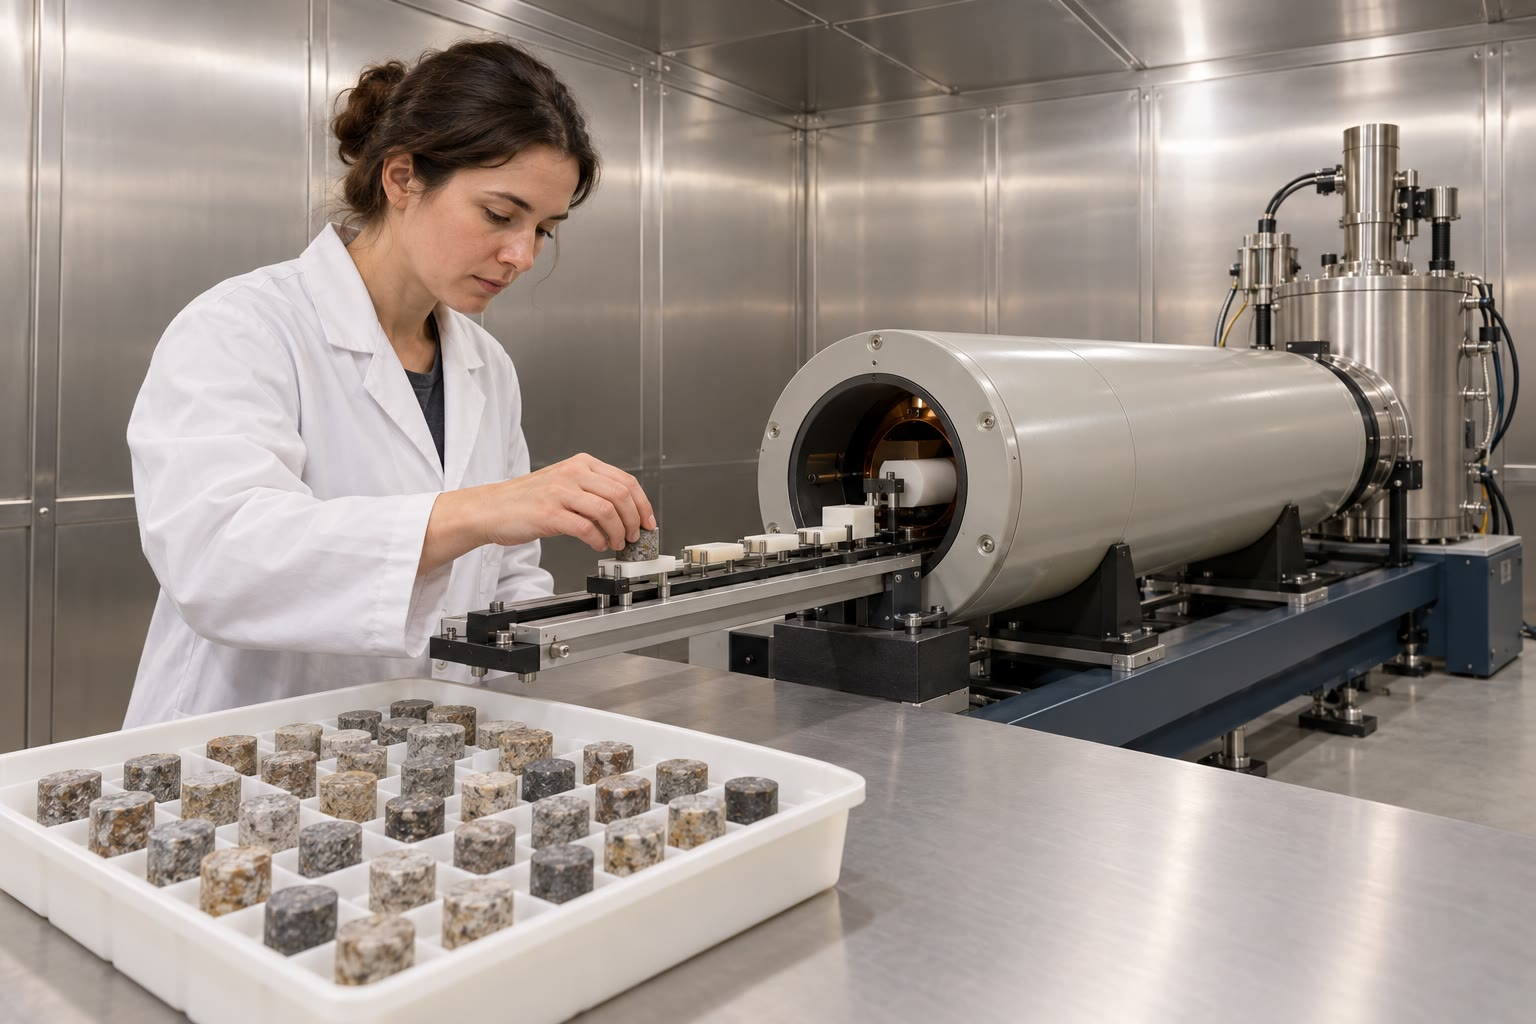
\includegraphics[width=\linewidth]{images/book5/ai/b3-palaeomag-lab.jpg}

{\scriptsize Het laden van monsters op de monsterlade van een magnetometer in een
afgeschermde ruimte (door AI gegenereerde illustratie).}
\end{minipage}
\end{inthelab}

\section{Oefeningen}

\begin{exercise}[$\star$]\label{exo:b3:palaeomagnetism:1}
Bereken in een geocentrisch axiaal dipoolveld de inclinatie op breedtegraad
\ang{30}~NB, en de breedtegraad van een locatie waar de inclinatie \ang{-20} is.
\end{exercise}

\begin{exercise}[$\star$]\label{exo:b3:palaeomagnetism:2}
Op een station heeft het veld de componenten $X = \qty{20000}{nT}$, $Y =
\qty{-2000}{nT}$ en $Z = \qty{40000}{nT}$. Bereken $H$, $F$, de magnetische
declinatie en de inclinatie.
\end{exercise}

\begin{exercise}[$\star$]\label{exo:b3:palaeomagnetism:3}
In 2025 geldt $g_1^0 = \qty{-29350}{nT}$. Neem het veld als een axiale dipool en
bereken het veld aan de evenaar en aan de polen, en het dipoolmoment
($a = \qty{6371.2}{km}$, $\mu_0 = 4\pi\times\qty{e-7}{H.m^{-1}}$).
\end{exercise}

\begin{exercise}[$\star$]\label{exo:b3:palaeomagnetism:4}
Benoem het soort remanentie dat wordt verworven en wanneer het het veld vastlegt, voor: (a) een lavastroom
die afkoelt; (b) silt die bezinkt in een rustig meer; (c) een zandsteen waarvan de
ijzeroxidecoatings tijdens de vroege begraving in hematiet veranderen; (d) een basalt
die een miljoen jaar in het huidige veld ligt.
\end{exercise}

\begin{exercise}[$\star\star$]\label{exo:b3:palaeomagnetism:5}
Vier monsters van een locatie geven de richtingen $(D, I)$: $(\ang{12}, \ang{48})$,
$(\ang{22}, \ang{44})$, $(\ang{16}, \ang{57})$ en $(\ang{6}, \ang{53})$.
Bereken hun eenheidsvectoren, de lengte van de resultante $R$, de gemiddelde richting, $k$
en $\alpha_{95}$.
\end{exercise}

\begin{exercise}[$\star\star$]\label{exo:b3:palaeomagnetism:6}
Een locatie op \ang{40.0}~NB, \ang{10.0}~OL geeft de gemiddelde richting $D = \ang{20}$,
$I = \ang{50}$. Bereken de \omterm{def:b3:palaeomagnetism:vgp}{paleobreedte} en de \omterm{def:b3:palaeomagnetism:vgp}{virtuele geomagnetische pool}.
\end{exercise}

\begin{exercise}[$\star\star$]\label{exo:b3:palaeomagnetism:7}
Het IGRF geeft een dipoolmoment van \qty{8.32e22}{A.m^2} in 1900 en
\qty{7.69e22}{A.m^2} in 2025, en een veranderingssnelheid van $g_1^0$ van
\qty{+12.6}{nT/yr} in 2025. (a) Bereken de relatieve verandering van het moment per
eeuw. (b) Als $g_1^0$ die snelheid zou behouden, na hoeveel jaar zou het nul bereiken?
Waarom is dit geen voorspelling?
\end{exercise}

\begin{exercise}[$\star\star$]\label{exo:b3:palaeomagnetism:8}
De resterende remanentie van een monster, in \unit{mA/m} (noord, oost, neer), is
$(32.2, 18.1, 38.2)$ na verhitting tot \qty{20}{\celsius}, $(25.8, 18.1, 24.6)$
na \qty{300}{\celsius}, en $(0.0, 0.0, 0.0)$ na \qty{580}{\celsius}; het
\omterm{def:b3:palaeomagnetism:zijderveld}{Zijderveld-diagram} is recht tussen elk paar. Bereken de richting en intensiteit van de component die
tussen 20 en \qty{300}{\celsius} wordt verwijderd, en van die welke boven
\qty{300}{\celsius} wordt verwijderd. Welke is de ChRM, en wat is de
andere?
\end{exercise}

\begin{exercise}[$\star\star$]\label{exo:b3:palaeomagnetism:9}
Een formatie geeft $I = \ang{-35}$ met $\alpha_{95} = \ang{5}$. Bereken de
\omterm{def:b3:palaeomagnetism:vgp}{paleobreedte}, het bereik van \omterm{def:b3:palaeomagnetism:vgp}{paleobreedtes} dat is toegestaan door $I \pm \alpha_{95}$,
en de halve assen $\mathrm dp$ en $\mathrm dm$ van de betrouwbaarheidsovaal van de
pool.
\end{exercise}

\begin{exercise}[$\star\star\star$]\label{exo:b3:palaeomagnetism:10}
(a) Bepaal uit \cref{thm:b3:palaeomagnetism:dipole} de breedtegraad waarop
de inclinatie \ang{45} is, en de verhouding van het veld aan de polen tot dat aan de
evenaar. (b) Toon aan dat $\mathrm dI/\mathrm d\lambda = 2/(1 + 3\sin^2\lambda)$,
en leid af waar een fout in de inclinatie de grootste fout in de
\omterm{def:b3:palaeomagnetism:vgp}{paleobreedte} oplevert. (c) Waarom zijn \omterm{def:b3:palaeomagnetism:vgp}{paleobreedtes} die uit lage inclinaties volgen het
nauwkeurigst uitgedrukt in graden?
\end{exercise}

\begin{exercise}[$\star\star\star$]\label{exo:b3:palaeomagnetism:11}
Een locatie ligt op \ang{35.0}\,Z, \ang{150.0}\,O op een stabiele plaat waarvan
de referentiepool, voor de ouderdom van een formatie die daar is bemonsterd, ligt op \ang{70.0}\,NB,
\ang{300.0}\,OL. (a) Bereken de hoekafstand $p$ van de locatie tot de pool,
de verwachte inclinatie en declinatie, en de verwachte \omterm{def:b3:palaeomagnetism:vgp}{paleobreedte}.
(b) De formatie geeft $D_o = \ang{30.0}$, $I_o = \ang{-60.0}$. Bereken de
rotatie $R$ en de poolwaartse verschuiving $P$, en zeg wat ze betekenen.
\end{exercise}

\begin{exercise}[$\star\star\star$]\label{exo:b3:palaeomagnetism:12}
(a) Toon uit \cref{prop:b3:palaeomagnetism:fisher} aan dat de kans dat
een richting binnen $\theta$ van het gemiddelde ligt, is gelijk aan $(e^\kappa -
e^{\kappa\cos\theta})/(e^\kappa - e^{-\kappa})$. (b) Toon voor grote $\kappa$ en
kleine $\theta$ aan dat dit ongeveer $1 - e^{-\kappa\theta^2/2}$ is, en leid af dat
\qty{63}{\percent} van de richtingen binnen $\theta_{63} \approx
\ang{81}/\sqrt\kappa$ ligt. (c) Bereken $\theta_{63}$ voor $\kappa = 50$, en controleer de
\qty{63}{\percent} met de exacte formule.
\end{exercise}

\section{Probleem: De roodbedden van Kesta}

\begin{problem}[{Weekendprobleem --- drie formaties van een verplaatst terrein,
hun richtingen, polen en rotaties, en de ouderdom van de jongste}]
\label{pb:b3:palaeomagnetism:1}
% values: calc/ch04.py; palaeomag_stats.py, magnetostratigraphy.py; GPTS: iodp:gpts2004
Kesta is een verzonnen terrein, nu op \ang{47.0}\,NB, \ang{15.0}\,OL, aan de rand
van een verzonnen stabiel continent. Het ontsluit drie roodbedformaties: A,
\qty{60}{Ma}; B, \qty{30}{Ma}; C, van ongeveer 3.7 tot \qty{2.4}{Ma}. Elk werd
op meerdere locaties bemonsterd, en elk specimen werd thermisch gedemagnetiseerd; de
ChRM wordt gedragen door hematiet, en de formaties liggen horizontaal.

\medskip\noindent\textbf{Deel I --- Gemiddelde richtingen.} De zes locaties van
formatie A geven $(D, I)$: $(\ang{50}, \ang{37})$, $(\ang{28}, \ang{37})$,
$(\ang{21}, \ang{42})$, $(\ang{24}, \ang{27})$, $(\ang{37}, \ang{39})$,
$(\ang{46}, \ang{38})$.
\begin{enumerate}
  \item Waarom kan een ChRM die door hematiet wordt gedragen in een roodbed jonger zijn dan de
        laag? Wat zou aantonen dat hij niet veel jonger is?
  \item Bereken de eenheidsvector van de eerste richting.
  \item De som van de zes eenheidsvectoren is $(3.8943, 2.6500, 3.5717)$. Bereken $R$ en
        de gemiddelde richting van formatie A.
  \item Bereken $k$ en $\alpha_{95}$ voor formatie A.
  \item Formatie B geeft, uit 7 locaties, $D = \ang{23.9}$, $I = \ang{51.5}$ en
        $R = 6.8979$; formatie C, uit 8 locaties, $D = \ang{3.4}$, $I =
        \ang{63.7}$ en $R = 7.8707$. Bereken $k$ en $\alpha_{95}$ van elk.
  \item Welke formatie is het best gegroepeerd? Welk gemiddelde is het best bepaald?
\end{enumerate}

\medskip\noindent\textbf{Deel II --- Paleobreedtes en polen.}
\begin{enumerate}[resume]
  \item Bereken de \omterm{def:b3:palaeomagnetism:vgp}{paleobreedtes} van A, B en C.
  \item Bereken voor formatie A de paleocolatitude $p$ en de breedtegraad van
        de \omterm{def:b3:palaeomagnetism:vgp}{virtuele geomagnetische pool}.
  \item Bereken de lengtegraad van die pool, en controleer welk geval uit
        \cref{thm:b3:palaeomagnetism:pole} van toepassing is.
  \item Bereken $\mathrm dp$ en $\mathrm dm$ voor de pool van A.
  \item De polen van B en C liggen op \ang{66.5}\,NB, \ang{135.6}\,OL en
        \ang{87.1}\,NB, \ang{139.1}\,OL. Beschrijf het pad van de drie polen
        als functie van de ouderdom.
\end{enumerate}

\medskip\noindent\textbf{Deel III --- De ouderdom van formatie C.} In formatie C,
vanaf de basis zijn de specimens omgekeerd tot \qty{4.2}{m}, normaal tot
\qty{14.8}{m}, omgekeerd tot \qty{19.7}{m}, normaal tot \qty{24.6}{m}, omgekeerd tot
\qty{29.2}{m} en normaal tot \qty{54.0}{m}, daarna omgekeerd tot de top bij
\qty{64.0}{m}. Een asslaag op \qty{22}{m} is gedateerd op ongeveer \qty{3.2}{Ma}. De
normale subchronen van polariteitschron C2An omvatten 3.596--3.330, 3.207--3.116 en
3.032--\qty{2.581}{Ma}.
\begin{enumerate}[resume]
  \item Koppel de polariteitszones aan de tijdschaal, met behulp van de asslaag.
  \item Bereken de accumulatiesnelheid tussen de eerste en de derde
        omkeringsgrens, en tussen de vierde en de zesde.
  \item Schat de ouderdom van de basis en de top van de sectie.
  \item Waarom is de snelheid een gemiddelde over honderdduizenden jaren, en wat
        zou haar kunnen doen veranderen?
\end{enumerate}

\medskip\noindent\textbf{Deel IV --- Tegen het stabiele continent, en de drift.} De
referentiepolen van het stabiele continent liggen op \ang{78.0}\,NB, \ang{190.0}\,OL
($A_{95} = \ang{3.0}$) bij \qty{60}{Ma}; \ang{83.5}\,NB, \ang{175.0}\,OL
($\ang{2.5}$) bij \qty{30}{Ma}; en \ang{87.5}\,NB, \ang{150.0}\,OL ($\ang{2.0}$)
bij \qty{4}{Ma}.
\begin{enumerate}[resume]
  \item Bereken de hoekafstand van Kesta tot de referentiepool van \qty{60}{Ma},
        en de verwachte inclinatie en \omterm{def:b3:palaeomagnetism:vgp}{paleobreedte}.
  \item Bereken de verwachte declinatie bij \qty{60}{Ma}.
  \item De verwachte richtingen bij 30 en \qty{4}{Ma} zijn $(\ang{2.9},
        \ang{60.0})$ en $(\ang{2.5}, \ang{63.6})$. Bereken de poolwaartse
        verschuiving $P$ van A, B en C.
  \item Bereken de rotatie $R$ van A, B en C.
  \item Bereken de fouten $\Delta D_o$ en $\Delta D_x$ voor A, en de fout
        van de rotatie.
  \item De fouten van $R$ voor B en C zijn \ang{13.8} en \ang{17.9}. Welke
        rotaties zijn significant op 95 procent?
  \item Beschrijf de geschiedenis van Kesta ten opzichte van het stabiele continent.
  \item Bereken de noordwaartse drift van Kesta sinds formatie A, ten opzichte van
        de rotatie-as, in graden en in kilometer
        (\qty{111.19}{km} per graad).
  \item Bereken de \omterm{def:b3:palaeomagnetism:vgp}{paleobreedtes} die zijn toegestaan door $I \pm \alpha_{95}$ voor
        formatie A, en neem als één standaardafwijking de halve breedte van dat
        interval gedeeld door 1.96. Geef de noordwaartse drift van Kesta sinds formatie
        A, in kilometer, met de bijbehorende standaardafwijking.
\end{enumerate}
\end{problem}
